\documentclass[usenames,dvipsnames,notes,11pt,aspectratio=169]{beamer}
\usepackage{ifthen}
\usepackage{xcolor}
\usepackage{pgfplots}
\usepackage{amsmath}
\usepackage{centernot}
\usepackage{pifont}
\usepackage{tabularx}
\usepackage{makecell}
\usepackage{cuted}
\usepackage{subcaption}
\usepackage{booktabs}
\usepackage{array}
\usepackage{textcomp}
\usepackage{setspace}
\usepackage{xspace}
\usepackage{tikz}
\usepackage{pdfcomment}
\newcommand{\pdfnote}[1]{\marginnote{\pdfcomment[icon=note]{#1}}}
%\newcommand{\pdfnote}[1]{}

\usepackage{pgfpages}
%\setbeameroption{show notes on second screen}


\input ../beamer-style
\input ../std-macros
\input ../macros

\AtBeginSection[]
{
    \begin{frame}
        \frametitle{Table of Contents}
        \tableofcontents[currentsection]
    \end{frame}
}
\parskip=10pt

\title[CSCI-GA.2590]{Semantics}
\author[He He]{He He
}
\institute[NYU]{New York University}
\date{November 3, 2021}

\begin{document}
\begin{frame}
\titlepage
\end{frame}

\section{Introduction to semantics}

\begin{frame}
    {Syntax vs semantics}
    \textbf{Syntax}: does the string belong to the language?

    \textbf{Semantics}: what is the meaning of the string?

    Examples in programming languages:

    Different syntax, same semantics
    $$
    2 + 3 \qquad 3 + 2
    $$

    Same syntax, different semantics
    $$
    3 \;/\; 2 \;\;\text{(Python 2.7)} \qquad 3 \;/\; 2 \;\;\text{(Python 3)}
    $$

    (Slide adapted from Stanford CS221 Lecture 16)
\end{frame}

\begin{frame}
    {Model-theoretic semantics}
    An \textbf{expression} is a string of mere symbols.

    A \textbf{model} defines meanings of symbols.

    The output of an expression with respect to a model is its \textbf{denotation}.
    \pdfnote{In other words, the expression denotes a value.}

    \begin{table}
        \begin{tabular}{p{5cm}ll}
            expression & model & denotation \\
            \midrule
            \texttt{3 + 2 * 4} & calculator & 11 \\
            \texttt{the red ball} & an image & the red ball in the image \\
            \texttt{SELECT Name FROM Student WHERE Id = 0;} & database & John \\
            \texttt{Book me a ticket from NYC to Seattle} & database & [action] \\
        \end{tabular}
    \end{table}

    We understand the expression if we know how to act (in a world).
\end{frame}

\begin{frame}
    {Natural language as expressions}
    Motivating applications:

    \beamerblue{Question answering}\\
    \begin{itemize}
        \item[] What is the profit of Mulan? 
        \item[] Who is the 46th president of the US?
    \end{itemize}

    \beamerblue{Personal assistant}\\
    \begin{itemize}
        \item[] Alexa, play my favorite song.
        \item[] Siri, show me how to get home.
    \end{itemize}

    \begin{itemize}
        \item But natural language is full of ambiguities
        \item Cannot be directly handled by a computer (unlike programming/formal languages)
    \end{itemize}
\end{frame}

\begin{frame}
    {Semantic analysis}

    \beamerblue{Goal}: convert natural language to meaning representation\\
    \begin{itemize}
        \item[] John likes fruits. (\emph{informal}) 
        \item[] $\forall x \; \textsc{Fruit}(x) \implies \textsc{Likes}(x, \textsc{John})$ (\emph{formal})
    \end{itemize}

    {Main tool}: first-order logic 

    Why logic?\\
    \begin{itemize}
        \item Unambiguity: one meaning per statement
        \item Knowledge: link symbols to knowledge (entities, relations, facts etc.) (\emph{Take in complex information})
        \item Inference: derive additional knowledge given statements  (\emph{Reason with the information})
    \end{itemize}
\end{frame}

\begin{frame}
    {Logic and semantics: example}
    Natural language: ``John likes Mary's friends''

    Logical form: $\forall x \;\textsc{Friends}(x, \textsc{Mary}) \implies \textsc{Likes}(x, \textsc{John})$

    \textbf{World model}: state of affairs in the world\\
    \begin{itemize}
        \item[] People = \pc{\text{John}, \text{Mary}, \text{Joe}, \text{Ted}}
        \item[] John is a friend of Mary.
        \item[] Joe is a friend of Mary.
    \end{itemize}

    Given the world model,\\
    \begin{itemize}
        \item Is $\textsc{Likes}(\textsc{Joe}, \textsc{John})$ true?
        \item What else can we infer from the statement? 
    \end{itemize}

    The value of the expression may change given a different world model.
\end{frame}
%
%%\begin{frame}
%%    {Applications}
%%    {Question answering} (given a database)\\
%%    \begin{itemize}
%%        \item[] What is the profit of Mulan? 
%%        \item[] Who is the 46th president of the US?
%%    \end{itemize}
%%
%%    {Robot navigation}\\
%%    \begin{itemize}
%%        \item[] Open the pod bay doors, HAL.
%%        \item[] Pick up all socks in the living room. 
%%    \end{itemize}
%%
%%    {Natural language interface}\\
%%    \begin{itemize}
%%        \item[] Alexa, play my favorite song.
%%        \item[] Siri, show me how to get home.
%%    \end{itemize}
%%\end{frame}
%
\section{Logical languages}

\begin{frame}
    {Propositional logic}

    A \textbf{proposition} is a statement that is either true or false.\\
    \textbf{Propositional logic} deals with propositions and their relations.

    Syntax of propositional language:\\
    \begin{itemize}
        \item \textbf{Propositional symbols}: a \textit{primitive} set of propositions
            \begin{itemize}
                \item[] $p_1$: John likes Mary
                \item[] $p_2$: John is a student
            \end{itemize}
        \item \textbf{Logical connectives}: rules to build up \textbf{formulas}
            \begin{table}
                \begin{tabular}{llll}
                    symbol & read & meaning & formula \\
                    \midrule
                    $\neg$ & not & negation & $\neg p$ \\
                    $\lor $ & or & disjunction & $p\wedge q$ \\
                    $\land $ & and & conjunction & $p\vee q$ \\
                    $\implies $ & implies / if then & implication & $p\implies q$\\
                    $\iff$ & equivalent to / iff & equivalence & $p\iff q $ 
                \end{tabular}
            \end{table}
            \pdfnote{Concept check: where are these true?}
        \item Parentheses: $($, $)$
    \end{itemize}
\end{frame}

\begin{frame}
    {Parsing a formula}
    How would you check if a formula is valid (i.e. grammatical)?

    A propositional formula is contructed by connecting propositions using the connectives.
    \begin{itemize}
        \item Formulas can be nested.
        \item Parentheses are used to disambiguate formulas.
    \end{itemize}

    Example:
    \begin{itemize}
        \item[] $((p\land q) \land \neg p)$
        \item[] $((p\lor q) \land r) \implies p)$
    \end{itemize}
    Try to draw the parse trees of the formulas.

\end{frame}

\begin{frame}
    {World model for propositional logic}
    Propositional symbols:\\
    \begin{itemize}
        \item[] $p_1=$ hot
    \item[] $p_2=$ John likes ice cream
    \item[] $p_3=$ John ate an ice cream
    \end{itemize}

    Formula: $p_1 \land p_2 \implies p_3$ (Is this true?)
    \pause

    The \textbf{world model} in propositional logic is an \emph{assigment} of truth values to propositional symbols.
    \begin{table}
        \begin{tabular}{c|cccccccc}
            & $m_1$ & $m_2$ &$m_3$ &$m_4$ &$m_5$ &$m_6$ &$m_7$ &$m_8$ \\
            \midrule
            $p_1$ & T & T &T &T &F &F &F &F \\
            $p_2$ & T & T &F &F &T &T &F &F \\
            $p_3$ & T & F &T &F &T &F &T &F \\
        \end{tabular}
    \end{table}
    In which world(s) is the above formula false?
\end{frame}

\begin{frame}
    {Meaning of a formula}
    Propositional symbols:\\
    \begin{itemize}
        \item[] $p_1=$ hot
        \item[] $p_2=$ John likes ice cream
        \item[] $p_3=$ John ate an ice cream
    \end{itemize}
    Formula: $p_1 \land p_2 \implies p_3$  \hspace{2em} \emph{Just symbols!}

    Semantics is given by \emph{interpreting}  the formula against a world model.

    A formula specifies \emph{a set of world models} where it is true.

    A set of formulas is a knowledge base (constraints on the world model).

    Making inference given formulas and the world model: take a course in AI.
\end{frame}

\begin{frame}
    {Limitations of propositional logic}
    How do we represent knowledge of a \emph{collection} of objects?

    ``Everyone who likes ice cream ate an ice cream.''\\
    \begin{itemize}
        \item[] $p_{\textsc{John}}$ (John likes ice cream) $\implies q_{\textsc{John}}$ (John ate an ice cream)
        \item[] $p_{\textsc{Joe}}$ (Joe likes ice cream) $\implies q_{\textsc{Joe}}$ (Joe ate an ice cream)
        \item[] $p_{\textsc{Alice}}$ (Alice likes ice cream) $\implies q_{\textsc{Alice}}$ (Alice ate an ice cream)
        \item[] $p_{\textsc{Carol}}$ (Carol likes ice cream) $\implies q_{\textsc{Carol}}$ (Carol ate an ice cream)
        \item[] $\ldots$
    \end{itemize}

    [\hspace{2em}] likes ice cream $\implies$ [\hspace{2em}] ate an ice cream

    Need a compact way to represent a collection of objects!
\end{frame}

\begin{frame}
    {First-order logic}
    First-order logic generalizes propositional logic with several new symbols:

    Represent objects:\\
            \begin{description}
                \item[Constants] Primitive objects, e.g. \text{John}
                \item[Variables] Placeholder for some object, e.g. $x$
                \item[Functions] A map from object(s) to an object, e.g. $\text{John} \rightarrow \text{John's farther}$
            \end{description}

    Group objects:\\
    \begin{description}
        \item[Predicate] Properties of a set of objects, e.g. students, couples
    \end{description}

    Quantify a (infinite) set of objects:\\
    \begin{description}
        \item[Quantifiers] Specify the number of objects with a certain property, e.g. \emph{all} people are mortal.
    \end{description}
\end{frame}

\begin{frame}
    {Constants, variables, functions}
    \textbf{Constants} refer to primitive objects such as named entities:\\
    \begin{itemize}
        \item[] \textsc{John}, \textsc{IceCream}, \textsc{Hot}
    \end{itemize}

    A \textbf{variable} refers to an unspecified object:\\
    \begin{itemize}
        \item[] $x,y,z$
        \item[] $\textsc{Student}(x)$
        \item[] $\textsc{Friends}(x, \textsc{John})$
    \end{itemize}

    A $n$-ary \textbf{function} maps $n$ objects to an object:\\
    \begin{itemize}
        \item[] $\textsc{Mother}(x)$
        \item[] $\textsc{Friends}(\textsc{Mother}(x), \textsc{Mother}(y))$
    \end{itemize}
\end{frame}

\begin{frame}
    {Predicates}
    %A \textbf{relation} is a set of $n$-tuples:\\
    %\begin{itemize}
    %    \item[] $\textsc{Student} = \pc{\textsc{John}, \textsc{Joe}, \textsc{Mary}}$
    %    \item[] $\textsc{Friends} = \pc{(\textsc{John}, \textsc{Mary}), (\textsc{Mary}, \textsc{John})}$
    %    \item[] $\textsc{Smaller} = \pc{(\textsc{Apple}, \textsc{Car}), (\textsc{Desk}, \textsc{Building})}$ (not symmetric)
    %\end{itemize}

    A \textbf{predicate} is an indicator function $P\colon X\rightarrow \pc{\text{true}, \text{false}}$.\\
    \begin{itemize}
        \item Describes properties of object(s)
        \item $P(x)$ is an atomic formula
        \item[] $\textsc{Student}(\textsc{Mary})$
        \item[] $\textsc{Smaller}(\textsc{Desk}, \textsc{Computer})$
        \item[] $\textsc{Friends}(\textsc{John}, \textsc{Mary}) \implies \textsc{Friends}(\textsc{Mary}, \textsc{John})$
    \end{itemize}
\end{frame}

\begin{frame}
    {Quantifiers}
    \textbf{Universal quantifier}  $\forall$:\\
    \begin{itemize}
        \item The statement is true for \emph{every} object
        \item $\forall x \;P(x)$ is equivalent to $P(A) \land P(B) \land \ldots$
        \item All people are mortal: $\forall x\; \textsc{Person}(x) \implies \textsc{Mortal}(x)$
    \end{itemize}

    \textbf{Existential quantifier}  $\exists$:\\
    \begin{itemize}
        \item The statement is true for \emph{some} object
        \item $\exists x \;P(x)$ is equivalent to $P(A) \lor P(B) \lor \ldots$
        \item Some people are mortal: $\exists x\; \textsc{Person}(x) \land \textsc{Mortal}(x)$
    \end{itemize}

    Order matters, e.g.,``everyone speaks a language'':
    \begin{itemize}
        \item[] $\forall x \exists y \; \textsc{speaks}(x, y)$
        \item[] $\exists y \forall x \; \textsc{speaks}(x, y)$
    \end{itemize}
    \pdfnote{
        Everyone speaks a language (but they can speak different languges).
        There is a single language that everyone speaks.
    }
\end{frame}

\begin{frame}
    {Syntax of first-order logic}
    \textbf{Terms} refer to objects:\\
    \begin{itemize}
        \item Constant symbol, e.g. \textsc{John}
        \item Variable symbol, e.g. $x$
        \item Function of terms, e.g. $\textsc{Mother}(x)$, $\textsc{Capital}(\textsc{NY})$
    \end{itemize}

    \textbf{Formula} evaluates to true or false:\\
    \begin{itemize}
        \item Predicate over terms is an atomic formula, e.g. \textsc{Student}(\textsc{Mother}(\textsc{John}))
        \item Connectives applied to formulas (similar to propositional logic)
            \begin{itemize}
                \item[] $\textsc{Student}(x) \quad\land\quad \textsc{Happy}(x)$
            \end{itemize}
        \item Quantifiers applied to formulas 
            \begin{itemize}
                \item[] $\forall x \;\textsc{Student}(x) \implies \textsc{Happy}(x)$
                \item[] $\exists x \;\textsc{Student}(x) \land \textsc{Happy}(x)$
            \end{itemize}
    \end{itemize}
\end{frame}

\begin{frame}
    {World model of first-order logic}
    How do we know if $\textsc{Friends}(\textsc{John}, \textsc{Mary})$ is true?

    World model of propositional logic: \blue{propositions}\\
    \begin{table}
        \begin{tabular}{ll}
            proposition & truthful value \\
            \midrule
            John is a friend of Mary & True\\
            John is a friend of Joe & False
        \end{tabular}
    \end{table}

    World model of first-order logic: \blue{objects and their relations}\\
    \begin{table}
        \begin{tabular}{ll}
            constant symbol & object \\
            \midrule
            \textsc{John} & $a$ \\
             \textsc{Mary} & $b$ \\
        \end{tabular}
    \end{table}
    \vspace{-1.5em}
    \begin{table}
        \begin{tabular}{ll}
            predicate symbol & set of $n$-tuples \\
            \midrule
            \textsc{Friends} & $\pc{(a,b), (b,a)}$ \\
        \end{tabular}
    \end{table}
\end{frame}

\begin{frame}
    {Graph representation of the world model}
\end{frame}

\begin{frame}
    {Summary}

    \textbf{Syntax} produces symbols and well-formed formulas.

    \textbf{Semantics} grounds symbols to a world and allows for evaluation of formulas.

    We have seen how it works for formal languages such as propositional logic and first-order logic.

    Next, formal language to natural language.
\end{frame}

\section{Semantic parsing}

\begin{frame}
    {System overview}
    \begin{description}[Logical form]
        \itemsep2em
        \item[Utterance] Linguistic expression.\\
            ``Call John, please.''
        \item[Logical form] Formal meaning representation of the utterance\\
            $\textsc{Call}(\textsc{John})$ \hspace{4em} \emph{program}
        \item[Denotation] Output of the meaning representation with respect to the model\\
            Calling XXX-XXX-XXXX ...\hspace{4em} \emph{execution result}
    \end{description}
    \pdfnote{
        utterance -> logical form: parser
    }
    \pdfnote{
        logical form -> denotation: executor
    }
\end{frame}

\begin{frame}
    {Translate NL to logical language}
    Key idea: \emph{compositionality}
    \begin{center}
    \begin{tikzpicture}
    \tikzset{level distance=30pt, sibling distance=50pt}
    \Tree [.S [.NP John ] [.VP reads ] ]
    \end{tikzpicture}
    \end{center}
    \begin{itemize}
        \item Sentence: $\textsc{Reads}(\textsc{John})$ (What's the denotation?)
        \item We would like to construct it recursively
            \begin{itemize}
                \item John: \textsc{John} (a unique entity)
                \item reads: a predicate (function) that takes an entity (one argument) 
            \end{itemize}
    \end{itemize}
\end{frame}

\begin{frame}
    {A brief introduction to lambda calculus}
    Lambda calculus / $\lambda$-calculus\\
    \begin{itemize}
        \item A notation for applying a function to an argument
              $$\lambda x.x^2+x$$
        \item A function that is waiting for the value of a variable to be filled
        \item Function application by $\beta$-reduction
            $$(\lambda x.x^2+x)(2) = 2^2+2 = 6$$
        \item Takes multiple arguments by ``currying''
            \begin{align*}
                (\lambda x.\lambda y.xy)(2) &= \lambda y.2y \\
                (\lambda x.\lambda y.xy)(3)(2) &= (\lambda y.2y)(3) = 6
            \end{align*}
    \end{itemize}
\end{frame}

\begin{frame}
    {Translate NL to logical language}
    Verbs are predicates \\
    \begin{itemize}
        \item reads: $\lambda x.\textsc{Reads}(x)$ (waiting for an NP)
        \item likes: $\lambda x.\lambda y.\textsc{Likes}(x,y)$ (waiting for two NPs)
    \end{itemize}
    \centering
            \begin{tikzpicture}
            \tikzset{level distance=30pt, sibling distance=40pt}
                \Tree [.S:$\onslide<2->{\color{blue}\textsc{Likes}(\textsc{John},\textsc{Mary})}$
                [.NP:${\color{blue}\textsc{John}}$ John ]
                [.VP:$\onslide<2->{\color{blue}\lambda x.\textsc{Likes}(x,\textsc{Mary})}$
                    [.V:$\onslide<2->{\color{blue}\lambda y.\lambda x.\textsc{Likes}(x,y)}$ likes ]
                    [.NP:${\color{blue}\textsc{Mary}}$ Mary ] ] ]
            \end{tikzpicture}
\end{frame}

\begin{frame}
    {Compositional semantics}
    Bottom up parsing:\\
    \begin{itemize}
        \item Start with the semantics of each word
        \item Combine semantics of spans according to certain rules 
            \begin{itemize}
                \item Associate a combination rule with each grammar rule
                    \begin{table}
                        \begin{tabular}{lll}
                            V:${\color{blue}\lambda y.\lambda x.\textsc{Likes}(x,y)}$ & $\rightarrow$ & likes\\
                            NP:${\color{blue}\textsc{John}}$ &$\rightarrow$& John\\ 
                            VP:${\color{blue}\alpha(\beta)}$ &$\rightarrow$& V:${\color{blue}\alpha}$ NP:${\color{blue}\beta}$\\
                            S:${\color{blue}\beta(\alpha)}$ &$\rightarrow$& NP:${\color{blue}\alpha}$ VP:${\color{blue}\beta}$
                        \end{tabular}
                    \end{table}
                \item Get semantics by function applcation
            \end{itemize}
        \item Lexical rules can be complex!
    \end{itemize}
\end{frame}

\begin{frame}
    {Quantification}
    \vspace{2em}
    \begin{center}
        John bought a book
    \end{center}
    \vspace{-1em}
    $\textsc{Bought}(\textsc{John}, \textsc{Book})$?

    ``book'' is not a unique entity! $\textsc{Bought}(\textsc{Mary}, \textsc{Book})$

    Correct logical form: $\exists x \textsc{Book}(x) \land \textsc{Bought}(\textsc{John}, x)$

    But what should be the semantics of ``a''? $\lambda P.\lambda Q. \exists x\; P(x) \land Q(x)$

    ``a book'': $\lambda Q. \exists x\; \textsc{Book}(x) \land Q(x)$. (Need to change other NP rules)

    What about ``the'', ``every'', ``most''? 

    We also want to represent tense: ``bought'' vs ``will buy''. (event variables)
\end{frame}

\begin{frame}
    {Learning from derivations}

    Text: John bought a book (utterance)\\
    Annotation: 
    \includegraphics[height=3cm]{figures/derivation}

    Use approaches from (discriminative) constituent parsing

    \pause
    Obstacles:\\
    \begin{itemize}
        \item Derivations are rarely annotated.
        \item Unlike syntactic parsing, cannot obtain derivations from logical forms.
        \item Spurious derivation: wrong derivations that reach the correct logical form.
    \end{itemize}
\end{frame}

\begin{frame}
    {Learning from logical forms}
    Text: John bought a book (utterance)\\
    Annotation: $\exists x \textsc{Book}(x) \land \textsc{Bought}(\textsc{John}, x)$ (logical form)

    {Key idea}: model derivation as a latent variable $z$ [Zettlemoyer and Collins, 2005]

    Learning: maximum marginal likelihood
    \begin{align*}
        \log p(y\mid x) &= \log\sum_z p(y,z\mid x) \\
        &= \log\sum_z \frac{\exp\p{\theta\cdot\Phi(x,y,z)}}
        {\sum_{z',y'} \exp\p{\theta\cdot\Phi(x,y',z')}}
    \end{align*}
    
    \begin{itemize}
        \item Need to learn both the lexicon and the model parameters (for CCG)
        \item Use EM algorithm (with approximation)
    \end{itemize}
\end{frame}

\begin{frame}
    {Learning from denotations}
    Text: What states border Georgia? \\
    Annotation: Alabama, Florida, North Carolina, South Carolina, Tennessee

    {Key idea}: model the logical form as a latent variable $z$ [Liang, 2013]

    \begin{figure}
        \includegraphics[height=6cm]{figures/framework}
        \caption{[Liang 2016]}
    \end{figure}
\end{frame}

\begin{frame}
    {Datasets}
    {Geo880}\\
    \begin{itemize}
        \item 880 questions and database queries about US geography
        \item ``what is the highest point in the largest state?''
        \item Compositional utterances in a clean, narrow domain
        %\item ~90\% accuracy
    \end{itemize}

    {ATIS}\\
    \begin{itemize}
        \item 5418 utterances of airline queries and paired logical forms
        \item ``show me information on american airlines from fort worth texas to philadelphia''
        \item More flexible word order but simpler logic
        %\item ~86\% accuracy
    \end{itemize}

    {Free917, WebQuestions}\\
    \begin{itemize}
        \item Questions and paired logical forms on Freebase
        \item Logically less complex but scales to many more predicates
    \end{itemize}
\end{frame}

\begin{frame}
    {Text to SQL}
    \begin{figure}
        \includegraphics[height=6cm]{figures/text2sql}
    \end{figure}
    (Slide from Victoria Lin)
\end{frame}

\begin{frame}
    {Challenges}
        Design the logical representation and grammar
        \begin{itemize}
            \item Expressivity vs computation efficiency
            \item Domain-specific vs domain-general 
            \item Interacts with annotation and learning
        \end{itemize}

        Learning from different supervision signals
        \begin{itemize}
            \item End-to-end (utterance to action)
            \item Reinforcement learning (robotics, visual grounding)
            \item Interactive learning (obtain user feedback)
        \end{itemize}
\end{frame}

\end{document}
